% Calibration of Probabilities -- SMML project report (Assignment 2).
%
% Build (from report/):   latexmk -pdf -jobname=report main.tex
%   (latexmk needs Perl; without it: pdflatex -jobname=report main.tex, bibtex report,
%    then pdflatex -jobname=report main.tex twice.)
%   -> writes report/report.pdf, which is committed. Or compile main.tex on
%      Overleaf (upload main.tex, refs.bib and ../figures/) and rename the PDF.
%
% Rules for the text:
%   - 5-10 pages, target 8.
%   - Every number must come from results/*.csv. Each number-bearing paragraph
%     has a "% source:" comment naming the CSV it comes from; keep them updated.
%     "On k of 10 seeds" counts compare rows of metrics_all.csv (or cal_size.csv /
%     train_vs_heldout.csv) with the same dataset, seed and model.
%   - Penalty arithmetic for exact 0/1 predictions: n_exact_01_wrong * 34.54 / n_test,
%     with n_test = 921 (Spambase) or 9,045 (Adult); 34.54 = -log(1e-15).
%   - Theory is taken from the course lecture notes in lectures/ (one refs.bib entry,
%     cb_lectures; the optional note of each citation names the lecture);
%     claims and quotes about the reference study are from
%     lectures/calibration.icml05.crc.rev3.pdf.

\documentclass[11pt,a4paper]{article}

% 2 cm margins -> text width 17 cm. Figures are included at \figw = 16 cm = 6.3 in, the
% width they were drawn at, so their fonts appear at their real size (9 pt).
\usepackage[margin=2cm]{geometry}
\newcommand{\figw}{16cm}
\usepackage[T1]{fontenc}
\usepackage{lmodern}
\usepackage{microtype}
\usepackage{amsmath,amssymb}
\usepackage{graphicx}
\usepackage{booktabs}
\usepackage{caption}
\usepackage{xcolor}
\usepackage[numbers,sort&compress]{natbib}
\usepackage[hidelinks]{hyperref}

\graphicspath{{../figures/}}
\captionsetup{font=small,labelfont=bf}

% Let tall figures share a page with text, and fill float pages with them,
% instead of piling them up at the end of the document.
\renewcommand{\topfraction}{0.9}
\renewcommand{\bottomfraction}{0.8}
\renewcommand{\textfraction}{0.1}
\renewcommand{\floatpagefraction}{0.75}
\setcounter{topnumber}{2}
\setcounter{totalnumber}{3}

% Notation used throughout.
\newcommand{\R}{\mathbb{R}}
\newcommand{\E}{\mathbb{E}}
\DeclareMathOperator{\logit}{logit}

\title{Calibration of Probabilities\\[0.3em]
  \large Statistical Methods for Machine Learning --- Assignment 2}
\author{Salman Askarov \\ Matriculation number 65829A \\
  Università degli Studi di Milano, A.Y.\ 2025/26}
\date{\today}

\begin{document}
\maketitle

% source: results/metrics_summary.csv (ECE), results/metrics_all.csv (seed-wise counts),
% results/cal_size.csv, results/train_vs_heldout.csv.
\begin{abstract}
  A classifier can be accurate while its probabilities are poor estimates of
  $\eta(x) = \Pr(Y = 1 \mid X = x)$. Following Niculescu-Mizil and Caruana, I measure this
  for logistic regression (LR) and random forests (RF) on Spambase and Adult, and correct
  it with Platt scaling and isotonic regression fitted on a held-out calibration set, all
  implemented from scratch. Over ten random splits, both calibrators lower the Brier score
  and expected calibration error (ECE) of RF on every split (ECE from 0.053 to 0.020 and
  0.017 on Spambase, from 0.024 to 0.012 and 0.010 on Adult) without changing accuracy or
  AUC, while LR needs little correction, as in the reference study. Isotonic regression has
  the lowest ECE but a worse log-loss than Platt scaling, because a few of its outputs are
  wrong and exactly 0 or 1. For the same reason it does not overtake Platt scaling on Adult
  even with 5,000 calibration examples. Calibrating RF on its training set is worse than
  not calibrating.
\end{abstract}

% =====================================================================
\section{Introduction}\label{sec:intro}

In binary classification, a probabilistic predictor is meant to estimate
$\eta(x) = \Pr(Y = 1 \mid X = x)$, the function that defines the Bayes optimal
classifier~\citep[Statistical Learning; Logistic Regression]{cb_lectures}. Accuracy only checks whether $\hat p(x)$
exceeds $\frac12$, and ROC AUC only the order of the predictions, so a model can be
accurate but \emph{miscalibrated}: of the cases where it says 0.9, perhaps only 70\% are
positive. As \citet{niculescu2005} put it, accuracy and AUC are not sufficient when the
probabilities themselves are used. An example is the spam loss of~\citep[Introduction]{cb_lectures}, which
charges 2 for a legitimate e-mail flagged as spam and 1 for the opposite mistake: its
optimal rule flags an e-mail when $\eta(x) > \frac23$, which requires $\hat p \approx \eta$.

Following \citet{niculescu2005}, I train LR and RF, correct them with Platt
scaling~\citep{platt1999} and isotonic regression~\citep{zadrozny2002} fitted on held-out
data, and evaluate them on two datasets over ten random splits. Two extra experiments
vary the size of the calibration set and fit the calibrators on the training set instead.

% =====================================================================
\section{Background}\label{sec:background}

\paragraph{Calibration.} Examples are independent draws from an unknown distribution, and
the Bayes optimal classifier for the zero-one loss predicts 1 if and only if
$\eta(x) \ge \frac12$~\citep[Statistical Learning]{cb_lectures}, so thresholding $\hat p$ at $\frac12$ is
justified only if $\hat p$ estimates $\eta$. Since $\eta$ is unknown, one checks instead
the weaker property of \emph{calibration}~\citep{degroot1983},
\begin{equation}\label{eq:calibration}
  \Pr\bigl(Y = 1 \mid \hat p(X) = q\bigr) = q \qquad \text{for all } q \in [0, 1],
\end{equation}
which $\hat p = \eta$ implies but which the constant base rate also satisfies. A
\emph{reliability diagram} plots, for $K$ bins of predictions, the fraction of positives
$\bar y_k$ against the mean prediction $\bar p_k$; a calibrated model lies on the diagonal.
The expected calibration error is the weighted distance from it,
% n_k: number of test points in bin k (equal-width bins of [0, 1]).
% Code: calib.metrics.reliability_bins, calib.metrics.ece.
\begin{equation}\label{eq:ece}
  \mathrm{ECE} = \sum_{k=1}^{K} \frac{n_k}{n}\,\bigl|\bar y_k - \bar p_k\bigr|, \qquad K = 10,
\end{equation}
with $n_k$ predictions in bin $k$. It depends on the binning.

\paragraph{Losses for probabilities.} The logarithmic and quadratic losses
of~\citep[Introduction]{cb_lectures} give, on a test set,
% Code: calib.metrics.log_loss, calib.metrics.brier.
\begin{gather}
  \mathrm{LL} = -\frac{1}{n}\sum_{i=1}^{n} \bigl[y_i \log \tilde p_i + (1 - y_i)\log(1 - \tilde p_i)\bigr],
  \qquad
  \mathrm{BS} = \frac{1}{n}\sum_{i=1}^{n} (p_i - y_i)^2, \label{eq:logloss}\\
  \tilde p_i = \min\bigl(\max(p_i, 10^{-15}),\, 1 - 10^{-15}\bigr). \nonumber
\end{gather}
Both are minimized in expectation by $\eta$. For the quadratic loss the Bayes optimal
prediction is $\E[Y \mid X = x] = \eta(x)$~\citep[Statistical Learning]{cb_lectures}. For the logarithmic loss of
$\sigma(g(x))$, i.e.\ the logistic loss of $g$, the Bayes optimal $g$ is the log-odds
$\ln\frac{\eta}{1 - \eta}$, so $\sigma(g^*) = \eta$~\citep[Logistic Regression]{cb_lectures}. Both thus reward
calibration and separation together, but they differ in range. The quadratic loss lies in
$[0, 1]$, so the Chernoff--Hoeffding bound controls its test estimate~\citep[Statistical Learning]{cb_lectures}.
The logarithmic loss is unbounded, which discourages predictions too close to 0 or
1~\citep[Introduction]{cb_lectures}: after clipping, a wrong prediction of exactly 0 or 1 costs
$-\log 10^{-15} \approx 34.5$, about a hundred times our models' average log-loss. For
forecasts with finitely many values $p_k$, the Brier score splits
exactly as
% Exact for forecasts with finitely many values; with binned continuous forecasts there
% are extra within-bin terms. Used only for interpretation, not computed.
\begin{equation}\label{eq:murphy}
  \mathrm{BS} =
  \underbrace{\tfrac{1}{n}\textstyle\sum_{k} n_k (p_k - \bar y_k)^2}_{\text{reliability}}
  \;-\; \underbrace{\tfrac{1}{n}\textstyle\sum_{k} n_k (\bar y_k - \bar y)^2}_{\text{resolution}}
  \;+\; \underbrace{\bar y (1 - \bar y)}_{\text{uncertainty}},
\end{equation}
where $\bar y$ is the overall fraction of positives. Recalibration targets the reliability
term, but a map that merges distinct forecasts also loses resolution.

\paragraph{Why the two models differ.} Logistic regression predicts $\sigma(w^\top x)$ by
minimizing the logistic loss plus $\frac{\lambda}{2}\lVert w\rVert^2$ against
overfitting~\citep[Logistic Regression]{cb_lectures}. Since the optimum of this loss is the log-odds, LR
estimates $\eta$ well when the log-odds are nearly linear in $x$ (small approximation
error) and $\lambda$ is small, and \citet{niculescu2005} find it well calibrated on most
problems. A tree routes $x$ to a leaf $\ell$, and here outputs the leaf's fraction of
positives $N_\ell^+/N_\ell$ rather than its majority label. Grown to pure leaves, a tree
overfits~\citep[Tree Predictors]{cb_lectures}. A random forest~\citep{breiman2001} averages $T = 500$ trees
grown on bootstrap samples with random feature subsets,
$\hat p_{\mathrm{RF}}(x) = \frac1T \sum_t \hat p_t(x)$. \citet{niculescu2005} explain why
the average avoids 0 and 1: near the ends of $[0, 1]$ the trees' variance produces
one-sided errors, since the forest predicts 0 only if every tree does. Feature subsetting
makes this effect strongest for RF. The result is an S-shaped reliability curve, below the
diagonal at low predictions and above it at high ones, which the paper observes for RF on
several of its problems.

\paragraph{Platt scaling and isotonic regression.} Both map a real score $s(x)$ to a
probability by a non-decreasing function fitted on held-out pairs $(s_i, y_i)$. Platt
scaling~\citep{platt1999} is logistic regression with the single feature $s$,
% Platt's original form: p = 1/(1 + exp(A s + B)) with A = -a, B = -b.
% Code: calib.calibration.PlattScaler.
\begin{equation}\label{eq:platt}
  \hat p = \sigma(a s + b), \qquad \sigma(z) = 1/(1 + e^{-z}),
\end{equation}
fitted by maximum likelihood ($A = -a$, $B = -b$ in Platt's notation); $a > 1$ pushes
probabilities away from $\frac12$ and $a < 1$ pulls them towards it. Isotonic
regression~\citep{zadrozny2002} fits the best non-decreasing step function in squared
error, computed by Pool Adjacent Violators (PAV,~\citep{ayer1955}):
% w_i: weights (1, or the count after merging tied scores). Code: calib.calibration.IsotonicCalibrator.
\begin{equation}\label{eq:isotonic}
  \hat m = \operatorname*{arg\,min}_{m \text{ non-decreasing}} \; \sum_{i=1}^{n} w_i \bigl(y_i - m(s_i)\bigr)^2 .
\end{equation}
In the decomposition of the risk into estimation error, approximation error and Bayes
risk~\citep[Statistical Learning]{cb_lectures}, Platt scaling has a small estimation error (two parameters) but a
nonzero approximation error unless the distortion is a sigmoid in $s$. Isotonic regression
is nonparametric~\citep[Consistency]{cb_lectures}: its approximation error vanishes as the
calibration set grows, but on small sets its estimation error is large. Accordingly,
\citet{niculescu2005} find Platt scaling better for sigmoid-shaped distortions and small
sets, and isotonic regression more powerful with enough data. Isotonic regression's end
steps are exactly 0 or 1 when the extreme calibration points share a label, and on its
fitting set each step equals its points' mean label, so the reliability term
of~\eqref{eq:murphy} vanishes there. Both maps are monotone: Platt scaling preserves the
AUC, isotonic regression changes it only through ties, and accuracy changes only where
the probability crosses $\frac12$.

\paragraph{Why a held-out calibration set.} A test error estimates the risk without bias
only if the predictor does not depend on the test data, and the training error of an
overfitting predictor underestimates its risk~\citep[Statistical Learning]{cb_lectures}. The same applies to the
data a calibrator is fitted on. Reusing the training set would ``introduce unwanted
bias'': for a model that separates its training set, the sigmoid becomes ``just a 0,1
function''~\citep{niculescu2005}. The calibration set therefore plays the role of the
development set of~\citep[Hyperparameter Tuning]{cb_lectures}: data withheld from training to fit a few extra
parameters.

% =====================================================================
\section{Datasets and protocol}\label{sec:protocol}

% source: results/datasets.csv (rows, features, positives, duplicates),
% results/missing_values.csv (missing per column), results/splits.csv (split sizes).
% The 13.2% positive share among the dropped Adult rows is from notebook 01 (Observations
% cell), recomputed from the raw OpenML data on 29 Oct 2026 (0.1323); not saved in a CSV.
% Paper's Adult setup (Table 2 of niculescu2005): 14/104 attributes, 25% positive,
% 4,000 training and 1,000 calibration examples.
\paragraph{Datasets.} Both come from OpenML (Table~\ref{tab:datasets}).
\textbf{Spambase}~\citep{spambase1999} has 4,601 e-mails with 57 numeric, skewed and
mostly-zero features (word and character frequencies, capital-letter runs), 39.4\% spam,
and 394 rows that duplicate another row. \textbf{Adult}~\citep{adult1996} is a census
extract with 6 numeric and 8 categorical features, and the task is to predict an income
above \$50K. I drop the 3,620 rows with a missing \texttt{workclass} (2,799),
\texttt{occupation} (2,809) or \texttt{native-country} (857), leaving 45,222 rows with
24.8\% positives. The dropped rows are only 13.2\% positive, a slight population shift.
Adult is also one of the paper's problems, with the same 104 encoded attributes, but there
models are trained on 4,000 examples and calibrated on 1,000.

\begin{table}[tbp]
  \centering
  \small
  \caption{Datasets and splits. \emph{Dropped}: rows with a missing value.
    \emph{Features}: numeric + categorical. \emph{Encoded}: columns after one-hot
    encoding (for Adult, 103 on seeds 3 and 7, where a category seen in a single row
    is not in the training set). The split sizes are the same for all seeds.
    Positive class: spam for Spambase, income \texttt{>50K} for Adult.}
  \label{tab:datasets}
  \setlength{\tabcolsep}{4pt}
  \begin{tabular}{lrrrcrrrrr}
    \toprule
    Dataset & Raw rows & Dropped & Rows & Features & Encoded & Positive
      & Train & Calibration & Test \\
    \midrule
    Spambase & 4,601 & 0 & 4,601 & 57 + 0 & 57 & 39.4\% & 2,761 & 919 & 921 \\
    Adult & 48,842 & 3,620 & 45,222 & 6 + 8 & 104 & 24.8\% & 27,133 & 9,044 & 9,045 \\
    \bottomrule
  \end{tabular}
\end{table}

% source: results/splits.csv; results/metrics_all.csv (columns C, min_samples_leaf;
% n_exact_01 of rf/uncalibrated on Spambase = unanimous votes: 95-117 on the seeds with
% min_samples_leaf = 1, 0-4 on the others).
\paragraph{Splits, preprocessing and models.} Each dataset is split 60/20/20 into
training, calibration and test sets, stratified by class (each class is shuffled by a
seeded generator and cut at 60\% and 80\%). Everything is repeated for seeds 0--9, which
fix the split, the folds and the forest, and I report mean $\pm$ sample standard deviation.
As suggested in~\citep[Introduction]{cb_lectures}, numeric columns are rescaled (standardized with training
statistics) and categorical ones binary-encoded (one-hot with the training categories; an
unseen category becomes all zeros). The models come from scikit-learn~\citep{pedregosa2011}.
LR has an L2 penalty of inverse strength $C \in \{10^{-3}, \dots, 10^{2}\}$, and RF has 500
trees, $\sqrt d$ features per split and \texttt{min\_samples\_leaf} $\in \{1, 3, 10\}$. The
hyperparameter is tuned by 5-fold stratified cross-validation on the training set
only~\citep[Hyperparameter Tuning]{cb_lectures}, scored by log-loss. LR chose $C = 1$ on all Spambase seeds and
$C \in \{0.1, 1\}$ (five seeds each) on Adult. RF chose \texttt{min\_samples\_leaf} $= 1$
(pure leaves) on 7 Spambase seeds, and $3$ on the other three and on all Adult seeds.

\paragraph{Scores, leakage and metrics.} The calibrators take the logit $w^\top x + c$ for
LR, and for RF the logit of the clipped vote,
% Code: calib.models.get_scores; unanimous votes give s = +-logit(1 - 1e-6) = +-13.8.
\begin{equation}\label{eq:rfscore}
  s_{\mathrm{RF}}(x) = \logit\bigl(\min(\max(\hat p_{\mathrm{RF}}(x), \delta),\, 1 - \delta)\bigr),
  \qquad \logit(q) = \log\tfrac{q}{1 - q}, \quad \delta = 10^{-6}.
\end{equation}
On the log-odds scale of $\eta$~\citep[Logistic Regression]{cb_lectures}, the identity is the case $a = 1$,
$b = 0$ of~\eqref{eq:platt}, so a calibrated model can be left unchanged and $a > 1$ is
the stretch RF needs. The clip keeps unanimous votes finite (on Spambase, 95--117 test
points on the seeds with \texttt{min\_samples\_leaf} $= 1$, 0--4 otherwise). Isotonic
regression depends only on the order of the scores. The training set is used for
preprocessing, fitting and tuning, the calibration set only for the calibrators, and the
test set only for the final metrics: accuracy (threshold $\frac12$), log-loss, Brier score,
ECE (10 equal-width bins, as in the paper) and ROC AUC. The \emph{uncalibrated} method is
the model's own \texttt{predict\_proba}. I also count test predictions that are exactly 0
or 1, and the wrong ones among them.

% =====================================================================
\section{Implementation}\label{sec:implementation}
% source for iteration counts: results/metrics_all.csv (column platt_n_iter: 8-11).
Apart from the base models and their grid search, everything is written in numpy
(\texttt{src/calib/}).

\paragraph{Platt scaling by Newton's method.} As in~\citep{platt1999}, the labels are
replaced by smoothed targets, the method's built-in control against
overfitting~\citep{niculescu2005}, which keep $(a, b)$ finite even for separable data. The
objective is the logistic loss of~\citep[Logistic Regression]{cb_lectures} with these soft labels, computed with
\texttt{logaddexp} so that it never overflows:
% N_+, N_-: positives and negatives in the calibration set.
\begin{equation}\label{eq:platt-loss}
  t_i = \begin{cases} \frac{N_+ + 1}{N_+ + 2}, & y_i = 1,\\[0.5ex] \frac{1}{N_- + 2}, & y_i = 0, \end{cases}
  \qquad
  F(a, b) = \sum_{i=1}^{n} \bigl[\log(1 + e^{z_i}) - t_i z_i\bigr], \quad z_i = a s_i + b.
\end{equation}
$F$ is convex in $\theta = (a, b)$. With $x_i = (s_i, 1)^\top$ and $p_i = \sigma(z_i)$,
% eta: the largest of 1, 1/2, 1/4, ... with F(theta + eta Delta) <= F(theta).
% Start: a = 0, b = log((N_+ + 1)/(N_- + 1)). Stop: ||eta Delta|| < 1e-10, or 100 iterations.
\begin{equation}\label{eq:newton}
  g = \sum_{i} (p_i - t_i)\, x_i, \qquad
  H = \sum_{i} p_i (1 - p_i)\, x_i x_i^\top + 10^{-12} I, \qquad
  \theta \leftarrow \theta - \eta\, H^{-1} g,
\end{equation}
starting from $a = 0$, $b = \log\frac{N_+ + 1}{N_- + 1}$. The step length $\eta$ is halved
until $F$ does not increase, and the loop stops when the step norm falls below $10^{-10}$.
Every run converged in 8 to 11 iterations.

\paragraph{Isotonic regression by PAV.} The pairs are stable-sorted by score, and tied
scores are merged (weight = count, value = mean label). PAV pushes each point onto a stack
of blocks and, while the top block's mean label is not larger than the one below, merges
the two. Each point is pushed and popped at most once, so the fit is $O(n)$ after the
sort. A new score receives the value of the last block starting at or before it
(\texttt{searchsorted}); scores below the first block receive the first value.

\paragraph{Metrics and verification.} The metrics
implement~\eqref{eq:ece}--\eqref{eq:logloss}, and the AUC uses the Mann--Whitney rank
statistic with average ranks for ties. 78 tests (\texttt{tests/}, the only place where
scikit-learn's calibration and metric modules are imported) check the metrics against
\texttt{sklearn.metrics} to $10^{-10}$, PAV against \texttt{sklearn.isotonic} on data with
ties, and Platt scaling without smoothing against an unregularized one-feature logistic
regression to $10^{-5}$. All seeds are explicit and the forest predicts single-threaded, so
\texttt{python run\_all.py} reproduces every result exactly.

% =====================================================================
\section{Results}\label{sec:results}
% All numbers: results/metrics_all.csv, results/metrics_summary.csv;
% figures from seed 0 (results/preds_*_seed0.npz).

\begin{table}[tbp]
  \centering
  \caption{Test metrics, mean $\pm$ sample standard deviation over 10 seeds.
    Lower is better for log-loss, Brier score and ECE; higher is better for accuracy
    and ROC AUC.}
  \label{tab:t1}
  % Generated by calib.plotting.make_table_t1() from results/metrics_summary.csv.
  \resizebox{\textwidth}{!}{\begin{tabular}{lllccccc}
\toprule
Dataset & Model & Method & Accuracy & Log-loss & Brier score & ECE & ROC AUC \\
\midrule
Spambase & LR & Uncalibrated & 0.9205 $\pm$ 0.0067 & 0.2485 $\pm$ 0.0232 & 0.0639 $\pm$ 0.0041 & 0.0349 $\pm$ 0.0051 & 0.9674 $\pm$ 0.0045 \\
Spambase & LR & Platt & 0.9178 $\pm$ 0.0074 & 0.2481 $\pm$ 0.0178 & 0.0660 $\pm$ 0.0033 & 0.0413 $\pm$ 0.0085 & 0.9674 $\pm$ 0.0045 \\
Spambase & LR & Isotonic & 0.9213 $\pm$ 0.0066 & 0.3006 $\pm$ 0.0733 & 0.0623 $\pm$ 0.0042 & 0.0227 $\pm$ 0.0047 & 0.9660 $\pm$ 0.0049 \\
\addlinespace
Spambase & RF & Uncalibrated & 0.9455 $\pm$ 0.0081 & 0.1726 $\pm$ 0.0143 & 0.0451 $\pm$ 0.0040 & 0.0533 $\pm$ 0.0101 & 0.9832 $\pm$ 0.0044 \\
Spambase & RF & Platt & 0.9457 $\pm$ 0.0084 & 0.1544 $\pm$ 0.0199 & 0.0407 $\pm$ 0.0042 & 0.0195 $\pm$ 0.0058 & 0.9832 $\pm$ 0.0044 \\
Spambase & RF & Isotonic & 0.9458 $\pm$ 0.0089 & 0.2035 $\pm$ 0.0778 & 0.0412 $\pm$ 0.0045 & 0.0170 $\pm$ 0.0063 & 0.9823 $\pm$ 0.0052 \\
\midrule
Adult & LR & Uncalibrated & 0.8481 $\pm$ 0.0033 & 0.3253 $\pm$ 0.0041 & 0.1041 $\pm$ 0.0016 & 0.0109 $\pm$ 0.0031 & 0.9051 $\pm$ 0.0026 \\
Adult & LR & Platt & 0.8479 $\pm$ 0.0034 & 0.3253 $\pm$ 0.0041 & 0.1040 $\pm$ 0.0015 & 0.0110 $\pm$ 0.0031 & 0.9051 $\pm$ 0.0026 \\
Adult & LR & Isotonic & 0.8483 $\pm$ 0.0034 & 0.3292 $\pm$ 0.0046 & 0.1043 $\pm$ 0.0014 & 0.0109 $\pm$ 0.0039 & 0.9046 $\pm$ 0.0024 \\
\addlinespace
Adult & RF & Uncalibrated & 0.8618 $\pm$ 0.0039 & 0.3106 $\pm$ 0.0047 & 0.0979 $\pm$ 0.0019 & 0.0244 $\pm$ 0.0043 & 0.9158 $\pm$ 0.0034 \\
Adult & RF & Platt & 0.8619 $\pm$ 0.0046 & 0.3064 $\pm$ 0.0056 & 0.0970 $\pm$ 0.0022 & 0.0119 $\pm$ 0.0041 & 0.9158 $\pm$ 0.0034 \\
Adult & RF & Isotonic & 0.8609 $\pm$ 0.0043 & 0.3131 $\pm$ 0.0120 & 0.0971 $\pm$ 0.0021 & 0.0103 $\pm$ 0.0028 & 0.9153 $\pm$ 0.0035 \\
\bottomrule
\end{tabular}
}
\end{table}

% source: results/metrics_summary.csv (means, stds); results/metrics_all.csv (seed-wise
% counts; columns platt_a, platt_b, n_exact_01, n_exact_01_wrong).
\paragraph{Random forest.} RF is the more accurate model (Table~\ref{tab:t1}) and the one
that gains most from calibration. Both calibrators lower its Brier score and ECE on all ten
seeds of both datasets: the ECE falls from 0.0533 to 0.0195 (Platt) and 0.0170 (isotonic)
on Spambase, and from 0.0244 to 0.0119 and 0.0103 on Adult. Platt scaling also lowers the
log-loss, from 0.1726 to 0.1544 on Spambase (on 9 of 10 seeds) and from 0.3106 to 0.3064
on Adult (on all 10), while isotonic regression raises the mean log-loss on both. This
agrees with \citet{niculescu2005}, where RF is mildly miscalibrated on several problems and
helped by calibration.

\paragraph{Logistic regression.} On Adult, LR is already calibrated, as in the paper: the
three methods agree within a fraction of a standard deviation (ECE 0.0109, 0.0110,
0.0109), and Platt scaling learns nearly the identity ($a = 0.99 \pm 0.04$,
$b = -0.02 \pm 0.04$). On Spambase (ECE 0.0349), isotonic regression lowers the ECE to
0.0227 and the Brier score from 0.0639 to 0.0623 on all ten seeds, while Platt scaling
worsens both (to 0.0413 and 0.0660, on 8 and 9 seeds). Its $a = 0.84 \pm 0.11$ pulls all
probabilities towards $\frac12$, the failure the paper reports for well-calibrated models,
where the sigmoid ``has difficulty fitting the predictions in the tails''. LR's remaining
miscalibration on Spambase (Figure~\ref{fig:reliability}) is not sigmoid-shaped, so Platt
scaling's approximation error dominates.

\paragraph{Why isotonic regression has a poor log-loss.} Its end blocks often contain one
class only, so it outputs exactly 0 or 1 on average for 243.8 (LR) and 283.1 (RF) of the
921 Spambase test points, and for 500.4 and 989.0 of the 9,045 Adult ones. Of these, 2.5,
1.7, 1.1 and 2.2 per seed are wrong, at 34.5 each. For Spambase LR this adds
$2.5 \times 34.5 / 921 = 0.094$ to the log-loss, more than the whole gap of 0.052 to the
uncalibrated model. The same holds in the other three cases (penalties 0.064, 0.0042,
0.0084 against gaps 0.031, 0.0039, 0.0025). This is the unboundedness of the logarithmic
loss~\citep[Introduction]{cb_lectures}. With no bound, no Hoeffding-type guarantee keeps its test estimate
stable~\citep[Statistical Learning]{cb_lectures}: the number of such mistakes varies from 0 to 7 between seeds,
and isotonic log-loss on Spambase has a standard deviation of 0.073 and 0.078. The Brier
score (at most 1 per mistake) and the ECE (bin averages) barely register these points.

\paragraph{Ranking and accuracy.} Platt scaling leaves the AUC unchanged to within
$5 \times 10^{-6}$. Isotonic regression lowers it by 0.0005 to 0.0014 on average, because
its ties count $\frac12$ in the Mann--Whitney statistic. Mean accuracy moves by at most
0.003, most for Platt scaling on Spambase LR ($0.9205 \to 0.9178$), where $a < 1$, $b < 0$
shift the score at which the probability crosses $\frac12$.

\begin{figure}[tbp]
  \centering
  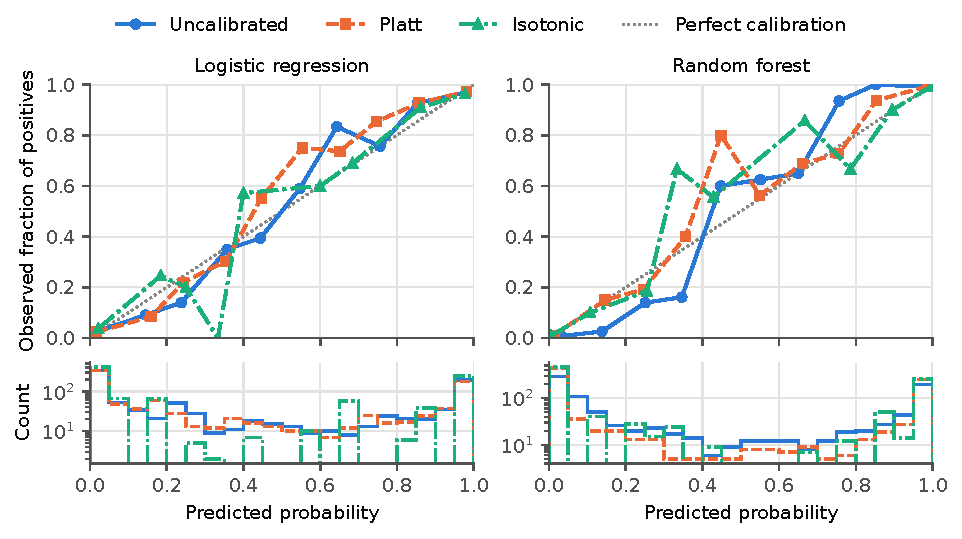
\includegraphics[width=\figw]{f1_reliability_spambase}\\[0.5ex]
  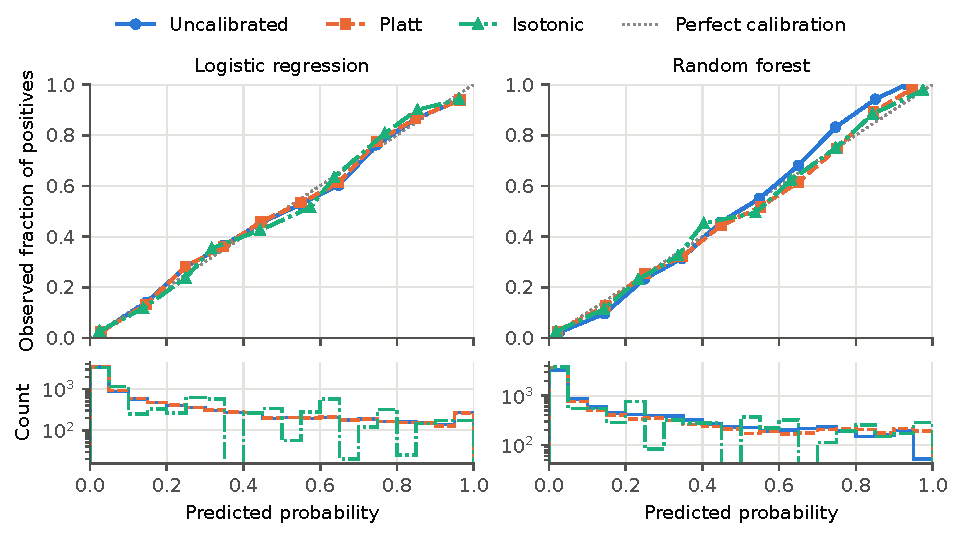
\includegraphics[width=\figw]{f1_reliability_adult}
  \caption{Reliability diagrams on the test set (seed 0), Spambase (top) and Adult
    (bottom), before and after calibration: fraction of positives against mean predicted
    probability in 10 equal-width bins (empty bins omitted); dotted: perfect calibration.
    Below each panel: histogram of the predictions (log scale).}
  \label{fig:reliability}
\end{figure}

\paragraph{Reliability diagrams.} On Spambase (Figure~\ref{fig:reliability}, one seed),
uncalibrated RF has the S-shape predicted by the variance argument: below the diagonal
under 0.4 and above it for most higher predictions. After calibration the curves cross the
diagonal back and forth. The rest is mostly noise, since the bins between 0.2 and 0.8 hold
only 15 to 40 test points each. On Adult, with ten times more points, the curves are
smooth. LR lies on the diagonal throughout, and RF lies above it over 0.5 (underconfident)
until calibration brings it back.

\begin{figure}[tbp]
  \centering
  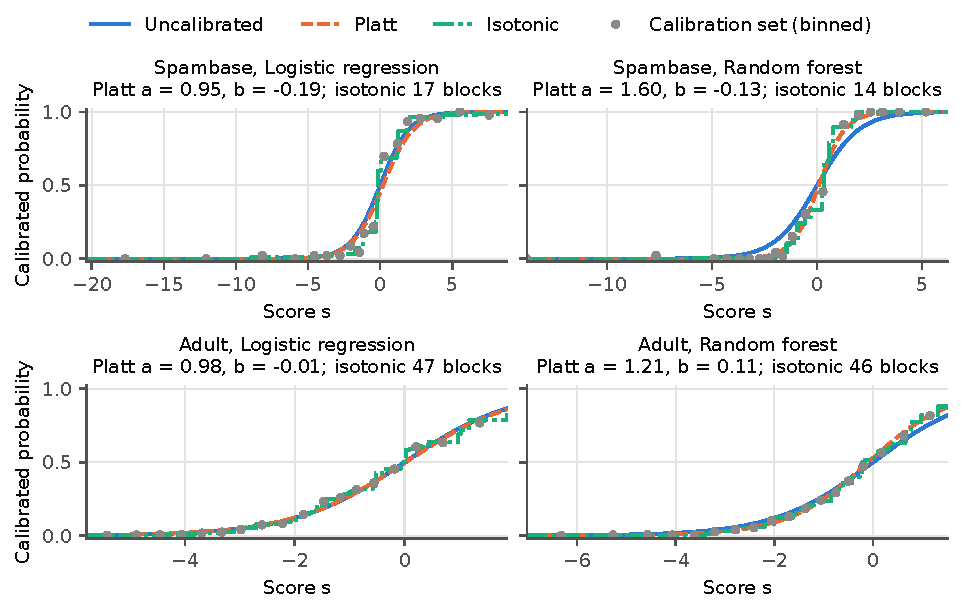
\includegraphics[width=\figw]{f2_correction_maps}
  \caption{Correction maps learned on the calibration set (seed 0): calibrated
    probability against score for Platt scaling and isotonic regression, with the
    uncalibrated map $\sigma(s)$ for reference. Grey dots: fraction of positives of the
    calibration set in score bins. Horizontal range: 5--95\% quantiles of the
    calibration scores.}
  \label{fig:maps}
\end{figure}

\begin{figure}[tbp]
  \centering
  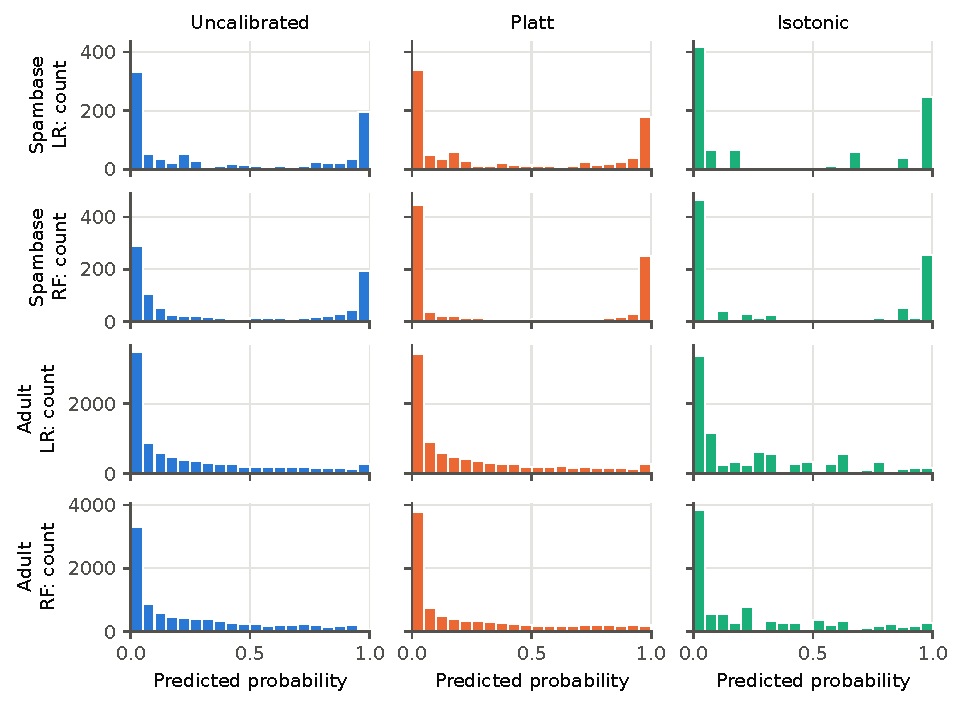
\includegraphics[width=\figw]{f3_histograms}
  \caption{Distribution of the predicted probabilities on the test set (seed 0),
    before calibration and after Platt scaling and isotonic regression.}
  \label{fig:histograms}
\end{figure}

% source: results/metrics_all.csv (columns platt_a, platt_b, iso_blocks).
\paragraph{Correction maps and predictions.} For RF the Platt sigmoid is steeper than
$\sigma(s)$ (Figure~\ref{fig:maps}): $a = 1.53 \pm 0.11$ on Spambase and $1.23 \pm 0.03$ on
Adult, with small intercepts ($b = 0.05 \pm 0.11$, $0.11 \pm 0.02$). It pushes the forest's
predictions away from $\frac12$, undoing the shrinkage caused by averaging. The isotonic
staircase follows the same trend, with 15.0 (RF) and 17.6 (LR) blocks on average on
Spambase against 42.9 and 44.7 on Adult (about 50--60 against 200 calibration points per
step), and its first and last steps are exactly 0 and 1 in all four seed-0 maps. As in the
paper, calibration extends RF's predictions into the tails (Figure~\ref{fig:histograms};
on Adult the top bin, almost empty before, fills up), Platt scaling gives smooth
histograms and isotonic regression coarse ones. Those few discrete values are the loss of
resolution in~\eqref{eq:murphy} and the ties that lower the AUC.

% source: results/metrics_summary.csv (stds, ECE), results/metrics_all.csv (platt_a).
\paragraph{Spambase vs Adult.} The calibration-set size (919 vs 9,044) controls the
estimation error of isotonic regression: the standard deviation of its log-loss is about
three (LR) and five (RF) times the uncalibrated one on Spambase, against 1.1 and 2.6 times
on Adult, while Platt scaling's stays close to it on both. Both models are more
miscalibrated on Spambase (uncalibrated ECE 0.053 vs 0.024 for RF, 0.035 vs 0.011 for LR).
My untested hypotheses are that the easier Spambase task has more cases with $\eta$ near 0
or 1, exactly where the variance argument pulls the forest inwards, and that its log-odds
are further from linear in the skewed frequency features, a larger approximation error
for LR.

% =====================================================================
\section{Extra experiments}\label{sec:extra}

\begin{figure}[tbp]
  \centering
  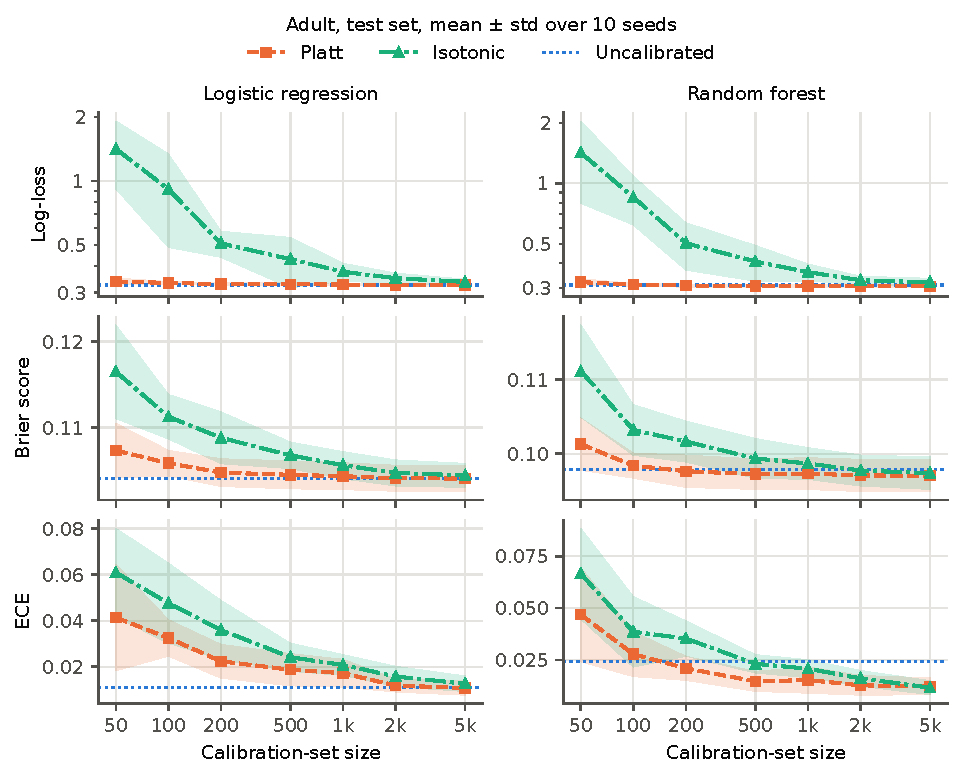
\includegraphics[width=\figw]{f4_calibration_size}
  \caption{Test log-loss, Brier score and ECE on Adult against the size of the
    calibration set (stratified subsamples of 50 to 5,000 examples), mean $\pm$ one
    standard deviation over 10 seeds. Dotted: uncalibrated model.}
  \label{fig:calsize}
\end{figure}

% source: results/cal_size.csv (means per model, method, cal_size; seed-wise platt vs
% isotonic). Penalty at 5,000: 4.4 * 34.54 / 9,045 = 0.017.
\paragraph{Size of the calibration set.} With the Adult base models fixed, the calibrators
are refitted on stratified subsamples of 50 to 5,000 examples (Figure~\ref{fig:calsize}).
\citet{niculescu2005} report, in squared error averaged over eight problems and nine
models, that Platt scaling wins below about 200--1,000 cases and that isotonic regression
is as good or better from 1,000. \textbf{On Adult the curves do not cross in log-loss or
Brier score.} Platt scaling is lower in log-loss on every seed at every size for both
models, and in Brier score on at least 9 of 10 seeds, although for RF at 5,000 the Brier
gap is small (0.0974 vs 0.0970). Isotonic regression improves fast, as a nonparametric
method should (RF log-loss 1.42 at 50 examples, 0.36 at 1,000, 0.32 at 5,000). At 5,000,
though, it is still above Platt scaling (0.3065) and the uncalibrated model (0.3106): its
4.4 wrong 0/1 outputs per seed cost about 0.017, more than the gap of 0.014. Only the ECE
converges as expected (RF at 5,000: 0.0117 vs 0.0124; at the full 9,044 isotonic regression
is ahead, 0.0103 vs 0.0119). I report this as a negative result, not a bug. My hypothesis is
that Adult's correction is nearly sigmoid in the logit (Figure~\ref{fig:maps}), so Platt
scaling's approximation error is small, the case in which the paper finds the methods
``virtually indistinguishable'' for large sets. The paper's other learning-curve findings
are reproduced. Calibrating an already calibrated model ``hurts performance when the
calibration sets are small'': with 50 or 100 examples, Platt scaling raises LR's ECE from
0.011 to 0.041 and 0.032. RF is helped ``once the calibration sets are large enough'':
about 200 examples for Platt scaling (log-loss and ECE), and 500 (ECE) or 2,000 (Brier
score) for isotonic regression.

\begin{figure}[tbp]
  \centering
  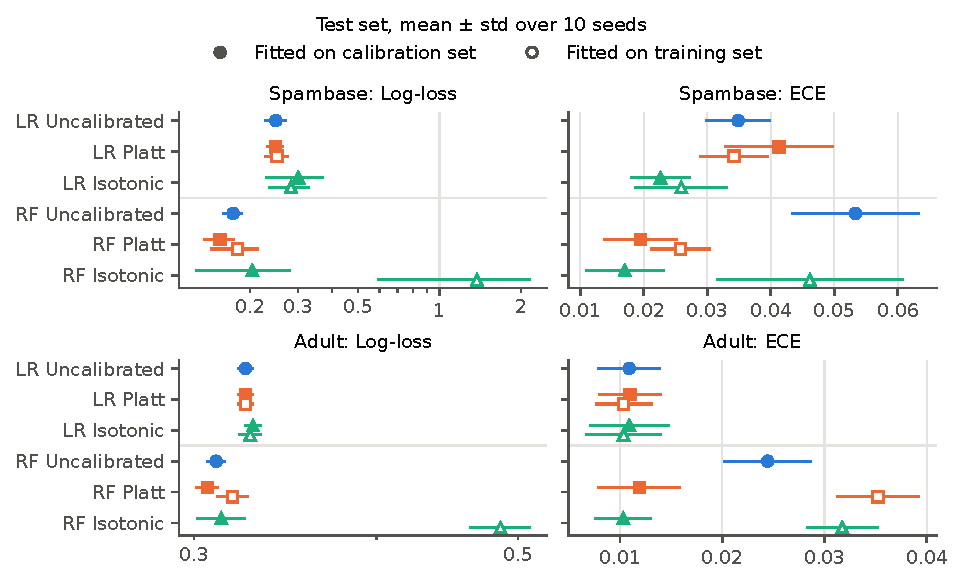
\includegraphics[width=\figw]{f5_train_vs_heldout}
  \caption{Test log-loss (log scale) and ECE when the calibrators are fitted on the
    training set (hollow markers) or on the held-out calibration set (filled markers),
    mean $\pm$ one standard deviation over 10 seeds.}
  \label{fig:trainheldout}
\end{figure}

% source: results/train_vs_heldout.csv (means per dataset, model, method, fit_on; seed-wise
% train vs cal). Penalty: 35.6 * 34.54 / 921 = 1.34. 63% = 1 - 1/e (bootstrap inclusion).
\paragraph{Calibrating on the training set.} Figure~\ref{fig:trainheldout} tests the
held-out argument of Section~\ref{sec:background}. For RF, fitting on the training set
worsens the test log-loss on every seed of both datasets for both calibrators, and on
average it is worse than no calibration. Each training point is in the bootstrap sample of
about 63\% of the trees, and with \texttt{min\_samples\_leaf} $= 1$ (most Spambase seeds)
those trees typically route it to a pure leaf of its own label~\citep[Tree Predictors]{cb_lectures}, so its
training vote is optimistic. A vote of 0.7 is almost always right on the training set, and
Platt scaling learns a much steeper map ($a = 2.69$ on Spambase and $1.75$ on Adult, against
$1.53$ and $1.23$ held out), which is overconfident on test data (Adult ECE 0.0353 against
0.0244 uncalibrated). Isotonic regression produces the paper's ``0,1 function'' almost
literally. On Spambase it keeps 6.3 blocks and outputs exactly 0 or 1 for 809.8 of the 921
test points, and the 35.6 wrong ones alone add $35.6 \times 34.5/921 = 1.34$ to a log-loss of
1.377. For LR the choice matters little: a regularized model with 57 or 104 weights fitted
on thousands of examples has a small estimation error, so its training scores look like its
test scores. On Spambase, Platt scaling fitted on the three times larger training set even
lowers the test Brier score on all ten seeds.

% =====================================================================
\section{Discussion and limitations}\label{sec:discussion}
% Hoeffding half-widths at delta = 0.05 for a [0,1] loss: sqrt(ln(2/0.05) / (2n)) =
% 0.045 (n = 921) and 0.014 (n = 9,045).
The results fit the bias--variance picture of Section~\ref{sec:background} and largely
reproduce the reference study. RF, an average of high-variance trees, is miscalibrated in
the predicted direction and should be recalibrated. Platt scaling on the logit of the vote
is a safe default: it improved all three probability metrics, needed only a few hundred
examples and never produced degenerate outputs. LR, whose loss is minimized by $\eta$
itself, should be recalibrated only if its reliability diagram shows a problem, and where
that problem is not sigmoid-shaped (Spambase), only the low-bias isotonic map helps. The
main departure from the paper is that the metric decides the verdict on isotonic
regression: best in ECE, worst in log-loss. Bounding its outputs away from 0 and 1 would
likely remove most of the penalty; I did not try it, to keep to the specified method.

\paragraph{Limitations.} (i)~Two datasets are a small basis compared with the paper's
eight. (ii)~The calibration set costs 20\% of the data; cross-validated calibration would
use all of it. (iii)~For a loss in $[0, 1]$, the Chernoff--Hoeffding bound~\citep[Statistical Learning]{cb_lectures}
gives a 95\% interval of $\pm 0.045$ on one Spambase test set and $\pm 0.014$ on Adult, wider
than most differences found. The evidence is therefore the consistency of the paired
comparisons over ten seeds, which is not a formal test, since the splits share data.
(iv)~The ECE depends on the binning and is noisy in Spambase's sparse middle bins.
(v)~Dropping Adult's incomplete rows (13.2\% positive) restricts the results to the
complete-case population, and Spambase's 394 duplicated rows can fall in both training and
test. (vi)~The RF score clip affects Platt scaling on unanimous votes, and the figures show
one seed.

% =====================================================================
\section{Conclusion}\label{sec:conclusion}
With Platt scaling (Newton's method), isotonic regression (PAV), the metrics and the data
pipeline implemented from scratch, I reproduced the main qualitative findings of
\citet{niculescu2005} on two datasets. The random forest is underconfident, with the
S-shaped reliability curve of averaged high-variance trees, and both calibrators fix most
of this without changing its ranking or accuracy. Logistic regression, whose loss is
minimized by $\eta$, needs little correction, and calibration must use held-out data.
Unlike the paper's averages, on Adult Platt scaling beat isotonic regression at every
calibration-set size tried, because the correction is nearly sigmoid and isotonic
regression's exact 0/1 outputs are heavily penalized by the unbounded logarithmic loss.

% =====================================================================
\section*{Declaration}
% Required verbatim. Do not edit the text.
I declare that this material, which I now submit for assessment, is entirely my own
work and has not been taken from the work of others, save and to the extent that such
work has been cited and acknowledged within the text of my work. I understand that
plagiarism, collusion, and copying are grave and serious offences in the university
and accept the penalties that would be imposed should I engage in plagiarism,
collusion or copying. This assignment, or any part of it, has not been previously
submitted by me or any other person for assessment on this or any other course of
study.

\bigskip
\noindent Salman Askarov \hfill \today

% =====================================================================
\bibliographystyle{plainnat}
{\footnotesize
\setlength{\bibsep}{1pt plus 1pt}
\bibliography{refs}}

\end{document}
